\section{Implementation}
\label{s:implementation}

\begin{figure}
    \centering
    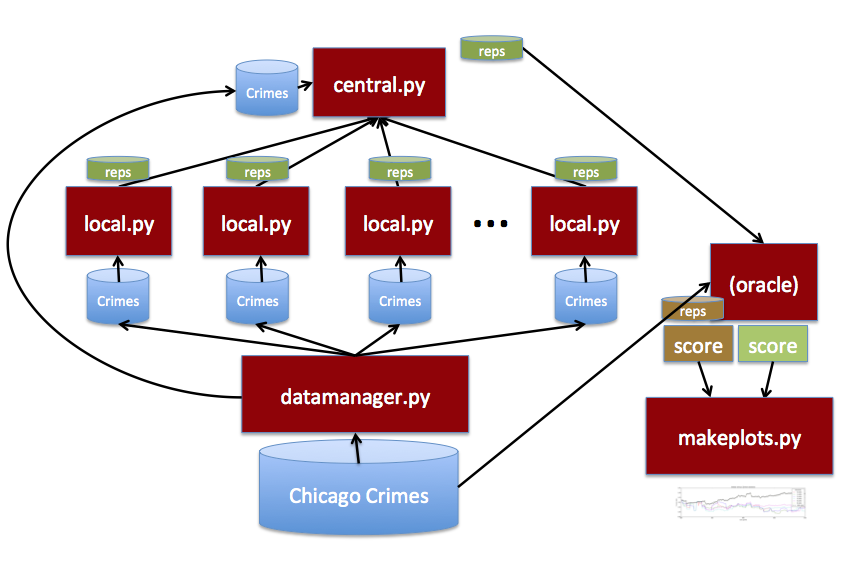
\includegraphics[width=\linewidth]{system}
    \caption{System diagram}
     \label{fig:implementation}
\end{figure}

The implementation of the system can be found at github.com/ericbalkanski/cs262project, and contains 5 python files that interact according to the diagram in figure \ref{fig:implementation}:
\begin{itemize}
    \item \texttt{datamanager.py} contains functions:
    \begin{itemize}
        \item \texttt{features}, used internally to preprocess data.
        \item \texttt{initialinsert}, which inserts data from the large crimes set to the local files read by local and central processes, selecting which file uniformly at random.
        \item \texttt{update}, which appends additional entries to these files at a set rate.
        \item \texttt{simulate}, which calls \texttt{initialinsert}, starts local and central processes, then calls \texttt{update}. It also performs oracle scoring, recording the performance of the central solution (read from logs) on the entire dataset and running the the greedy algorithm run on the whole set by providing a local process with a file containing all data in the system. 
    \end{itemize}
    \item \texttt{local.py} contains the single function \texttt{local}, which monitors a data file for updates, recalculates representatives each time that file is updated, and sends its representatives (and process ID number) to the central process using sockets when enough changes have occurred since its last communication. On each update, the system time, number of local data points, and local score are recorded.
    \item \texttt{central.py} contains a single function \texttt{central}, which receives data over a socket from several local processes. When this happens, it selects from its received representatives those that best represent the contents of its data file and writes them to logs, along with system time, number of data points, and local score.
    \item \texttt{makeplots.py} can be called from the command line and reads central and oracle logs to produce plots of their raw scores and the ratio of the oracle score to each central process' score, per update.
    \item \texttt{greedy.py} contains several functions implementing the greedy algorithm of \citet{mirzasoleiman2013distributed}. The two that are called by other components are:
    \begin{itemize}
        \item \texttt{greedy}, which returns the representatives and their score for a dataset.
        \item \texttt{score}, which only returns the score. This is used to score the central representatives on the complete dataset.
    \end{itemize}
\end{itemize}

Experiments are run by calling \texttt{datamanager.simulate} with the desired parameters, and the plots shown in section \ref{s:experiments} are generated from the resulting logs by calling \texttt{makeplots}.

\vspace{3em}
\begin{table}
\begin{tabular}{l|l}
Module or Function & Purpose in our System \\
\hline
    \texttt{socket} & sends messages between local and central machines \\
    \texttt{json} & encodes data to be sent over wire \\
    \texttt{itertools.islice} & allows access to parts of files\\
    \texttt{random.randint} & generates random integers for machine selection\\
    \texttt{random.random} & generates random floats between 0 and 1, for deletion\\
    \texttt{time.sleep} & allows pause before and between updates\\
    \texttt{time.time} & allows system time in logs\\
    \texttt{os.rename} & allows swap file for deleting entries\\
    \texttt{csv.reader} & separates data elements without splitting on commas within quoted strings, as are found in our data\\
    \texttt{multiprocessing} & starts local, central, and oracle simulations\\
    \texttt{copy} & for manipulating list values
\end{tabular}
\caption{Imported code}
\label{tab:modules}
\end{table}
\vspace{3em}

The system is built on top of a number of pre-existing components. The details are can be found in the documentation of each function, but a brief summary of the functions and modules imported can be found in table \ref{tab:modules}. 
